\documentclass[10pt,twocolumn,letterpaper]{article}

\usepackage{cite}
\usepackage{caption}
\usepackage{underscore}
\usepackage{cvpr}
\usepackage{times}
\usepackage{epsfig}
\usepackage{graphicx}
\usepackage{amsmath}
\usepackage{amssymb}
\usepackage[utf8]{inputenc}
\usepackage[T1]{fontenc}
\usepackage{lmodern} % load a font with all the characters

% Include other packages here, before hyperref.

% If you comment hyperref and then uncomment it, you should delete
% egpaper.aux before re-running latex.  (Or just hit 'q' on the first latex
% run, let it finish, and you should be clear).
\usepackage[breaklinks=true,bookmarks=false]{hyperref}

\cvprfinalcopy % *** Uncomment this line for the final submission

\def\cvprPaperID{****} % *** Enter the CVPR Paper ID here
\def\httilde{\mbox{\tt\raisebox{-.5ex}{\symbol{126}}}}

% Pages are numbered in submission mode, and unnumbered in camera-ready
%\ifcvprfinal\pagestyle{empty}\fi
\setcounter{page}{1}
\begin{document}

%%%%%%%%% TITLE
\title{Laboratorio 5: Segmentación en BSDS500}

\author{Rafael Cuperman Coifman\\
Universidad de los Andes\\
Bogotá, Colombia\\
{\tt\small r.cuperman675@uniandes.edu.co}
% For a paper whose authors are all at the same institution,
% omit the following lines up until the closing ``}''.
% Additional authors and addresses can be added with ``\and'',
% just like the second author.
% To save space, use either the email address or home page, not both
}

\maketitle
%\thispagestyle{empty}

%%%%%%%%% ABSTRACT
\begin{abstract}
 En este experimento se efectúa la comparación cuantificada de tres diferentes métodos de segmentación, siendo dos de ellos muy básicos (kmeans y jerárquico) y otro más avanzado y actual (UCM). Además de esto se evalúan las diferencias entre representar a la imagen en dos espacios de color distintos (L*a*b* y RGB) para lograr dichas segmentaciones. Se evalúan los resultados en una gráfica de precisión contra cobertura, obteniendo el \textit{F-measure} para cada caso. Los resultados muestran que en L*a*b* es mejor que RGB sobre la base de datos utilizada y que UCM es tiene un mejor desempeño que la segmentación jerárquica y esta a su vez que la segmentación por kmeans para la base de datos tenida en cuenta. 
\end{abstract}

%%%%%%%%% BODY TEXT
\section{Introducción}

La segmentación de imágenes es un problema altamente estudiado por diferentes investigadores alrededor del mundo desde hace muchos años. El objetivo final de este problema es obtener las regiones que delimitan a los objetos dentro de una imágen cualquiera. Para esto se han desarrollado una gran variedad de algoritmos, desde unos más sencillos (con resultados aceptables), hasta otros mucho más complejos (con resultados excelentes). BSDS500 es una base de datos construída por Berkeley sobre la cuál se pueden hacer pruebas de diferentes algoritmos para evaluar y comparar sus desempeños. En este informe se presenta la comparación de 4 métodos: tres sencillos, implementados por el autor y uno más complejo, desarrollado por investigadores de Berkeley (UCM) \cite{UCM}.

%-------------------------------------------------------------------------
\subsection{Espacios de color \cite{Forsyth}} 

Existe una gran variedad de espacios de color para representar una imagen. Dado que en este proyecto sólo se utilizaron RGB y L*a*b*, se presenta un pequeño resumen de únicamente estos dos espacios.

\subsubsection{RGB}
El espacio de color RGB es el espacio más conocido y el que trae por defecto casi siempre una imagen a color. Una imagen con esta codificación representará cada píxel de ella por tres números (o canales) que van de 0 a 255. Estos tres canales son R(Rojo), G(Verde) y B(Azul). De esta manera el color de cada píxel se encuentra como una combinación de diferentes intensidades de rojo, verde y azul. Este espacio de color tiene varios problemas, donde dos principales son: (1) es imposible representar la totalidad de los colores naturales percibidos por los humanos con valores positivos de estos tres canales y (2) los colores no son perceptualmente unniformes, lo cual quiere decir que la distancia visual entre colores no es proporcional a la distancia en ese espacio de tres canales RGB.

\subsubsection{L*a*b*}
El espacio de color L*a*b* se construyó pensando en solucionar los dos problemas mencionados en el caso RGB, menteniendo una explicación conceptual de cada uno de los tres canales. En este espacio de color cada píxel también se representa por tres canales (L, a, b), donde cada uno tiene únicamente valores positivos. El canal L corresponde a la imagen en escala de gris de la imagen, es decir, corresponde a su luminosidad; el canal a varía de rojo puro a verde puro; y el canal b varía de amarillo puro a azul puro. 

Al solucionar el segundo problema mencionado del espacio RGB, el espacio de color es conocido como un espacio L*a*b* se le llama un espacio perceptualmente uniforme, donde las distancias visuales entre colores se representan de mucha mejor manera con distancias euclídeas en este espacio. 

\subsection{Métodos de segmentación  \cite{Szeliski}}

A manera de comparar el resultado del algoritmo UCM, propuesto por investigadores de Berkeley, con otros algoritmos mucho más sencillos, se escogieron dos métodos básicos: kmeans y segmentación jerárquica.

\subsubsection{KMeans}
KMeans es uno de los métodos de clustering más elementales. Este algoritmo busca agrupar pixeles en grupos de acuerdo a semejanzas entre ellos. Antes de construir estos clusters, se representa cada píxel de una manera predefinida dependiendo del problema. Como en este caso la idea es separar píxeles de acuerdo a sus colores, se puede representar cada píxel por tres valores correspondientes a sus tres canales en el espacio de color. Otras opciones es añadir además la coordenada de cada píxel o trabajar con texturas, entre otros. 

Este algoritmo empieza con la introducción, por parte del usuario, de cuántos grupos \textit{k} se quieren construir para agrupar los píxeles. El algoritmo asigna \textit{k} puntos (llamados centroides), generalmente al azar, en la imagen y mira la distancia de cada píxel a estos centroides, asignandole a cada píxel el centroide a cuya distancia es menor. Una vez se hace esto con todos los píxeles se calcula el centro de masa de cada uno de los \textit{k} grupos, siendo estos los nuevos centroides. Se repite el proceso con estos nuevos centroides hasta que haya convergencia. 

De esa manera se obtienen la separación de la imagen en \textit{k} grupos distintos. Esta separación puede considerarse como una segmentación, ya que cada cluster puede interpretarse como una sección de la imagen.

\subsubsection{Segmentación jerárquica}
La segmentación jerárquica es un método de segmentación un poco más complejo que KMeans, ya que produce una jerarquía de segmentaciones en forma de dendograma. Al igual que en kmeans, el primer paso corresponde en representar cada píxel como un vector de características, siendo en este caso el valor en cada uno de los tres canales de su espacio de color. Como ya se mencionó, esta representación varía de acuerdo a la imagen y al problema que se quiere solucionar.

La segmentación jerárquica tiene dos enfoques: ascendente y descendente. En este caso se presenta el enfoque ascendente, en la cual cada píxel se considera como un grupo por separado al principio y luego se juntan píxeles cercanos (según sus distancias en la representación escogida) para formar grupos más grandes. Para lograr este proceso de "unir" grupos, es necesario hallar las distancias entre todos los píxeles (según sus representaciones en vectores), lo cual puede ser computacionalmente costoso y lento. Al unir iterativamente grupos pequeños para formar grupos más grandes, se construye una estructura en forma de árbol llamada dendograma. A partir de esta se puede construir una segmentación. En la figura~\ref{fig:dendograma} se muestra un ejemplo de un dendograma. En esta estructura en la parte inferior se muestran todos los grupos iniciales (los más pequeños, siendo generalmente cada uno de los píxeles) y en la parte superior se encuentra la agrupación de todos los píxeles en un único grupo.

\begin{figure}[h]
    \centering
    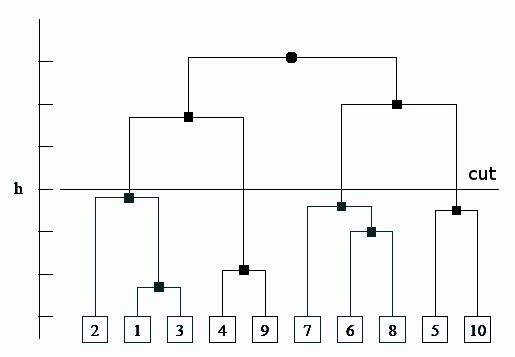
\includegraphics[width=0.5\textwidth]{Dendograma.jpg}
    \caption{Dendograma.\\Tomado de: http://svgopen.org/2010/papers/2-				Clustering_SVG_Shapes/dendroSelfBWcut.jpg}
    \label{fig:dendograma}
\end{figure}

Como fue mencionado, a partir de un dendograma es posible construir una segmentación de la imagen. Esto se logra "cortando" la estructura en un nivel escogido por el usuario. En el caso de la figura~\ref{fig:dendograma}, si se hace un corte en el nivel \textit{h}, como es mostrado, se generarán 4 clusters, donde en el primero estarán los píxeles 2,1 y 3; en el segundo los píxeles 4 y 9; en el tercero los píxeles 7, 6 y 8; y en el cuarto los píxeles 5 y 10.


%------------------------------------------------------------------------
\section{Desarrollo}

Para comparar las segmentaciones realizadas con los dos métodos anteriormente mencionados (jerárquico, y Kmeans) y UCM en la base de datos BSDS500, se desarrolló un código en Matlab que permitió escoger el espacio de color, el método de segmentación y la cantidad de clusters. Se escogieron tres combinaciones de método/espacio de color para comparar:

\begin{itemize}
	\item Segmentación por kmeans en espacio de color RGB.
    \item Segmentación por kmeans en espacio de color L*a*b*.
    \item Segmentación jerárquica en espacio de color L*a*b*.
\end{itemize}

Se escogió primordialmente el espacio de color L*a*b* ya que, como fue mencionado, este es un espacio perceptualmente uniforme, y como la segmentación se iba a hacer por colores de píxeles, se esperaba un mejor resultado con este espacio. Para verificar esta suposición se evaluó también con kmeans en el espacio RGB a modo de comparación de espacio de color.

\subsection{Segmentación}

\begin{figure}[h]
    \centering
    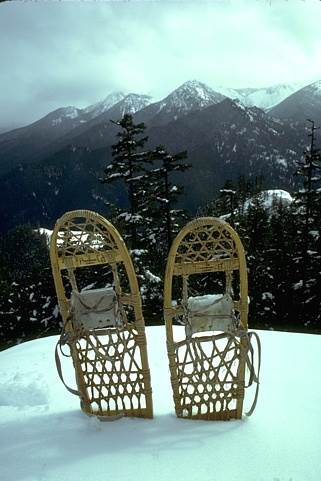
\includegraphics[width=0.2\textwidth]{Original.jpg}
    \caption{Imagen original de ejemplo}
    \label{fig:original}
\end{figure}

La segmentación se efectuó con una función implementada en Matlab, como ya fue mencionado. 

Se segmentaron las 200 imágenes con cada combinación método/espacio de color con 7 diferentes números de clusters (2, 3, 5, 8, 10, 15 y 20), obteniendo así 7 diferentes segmentaciones (cada una de mayor o menor nivel), para cada una de las 200 imágenes, por cada una de las 3 combinaciones seleccionadas. Es decir, se produjeron \(200 \times 7 \times 3 = 4200\) segmentaciones diferentes.

La función en Matlab permitió segmentar con diferentes métodos y en distintos espacios de representación. En las figuras ~\ref{fig:jerarquica}, ~\ref{fig:gmm}, ~\ref{fig:kmeans} y ~\ref{fig:watersheds} se muestran diferentes segmentaciones alcanzadas con la función implementada para la figura ~\ref{fig:original}


\begin{figure}[h]
    \centering
    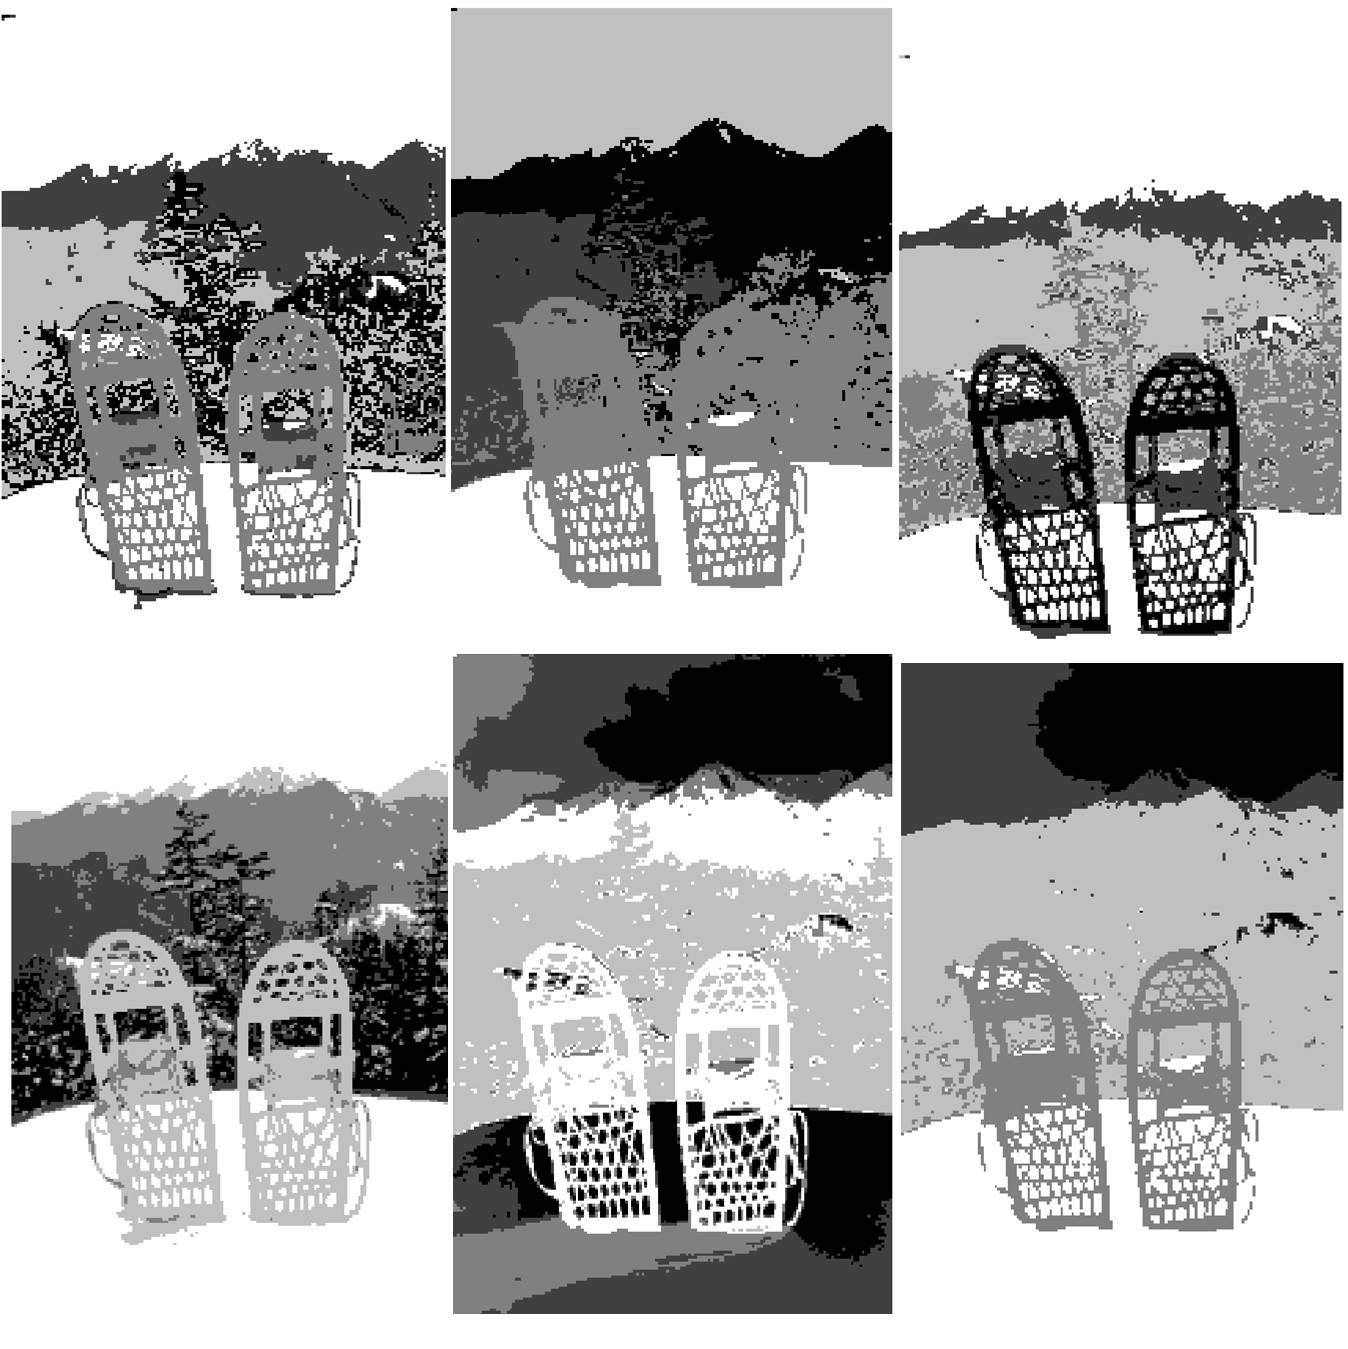
\includegraphics[width=0.4\textwidth]{Jerarquica.jpg}
    \caption{Segmentaciones jerárquicas para diferentes representaciones con 5 clusters: De izquierda a derecha de arriba a abajo: HSV, HSV+XY, LAB, LAB+XY, RGB, RGB+XY.}
    \label{fig:jerarquica}
\end{figure}

\begin{figure}[h]
    \centering
    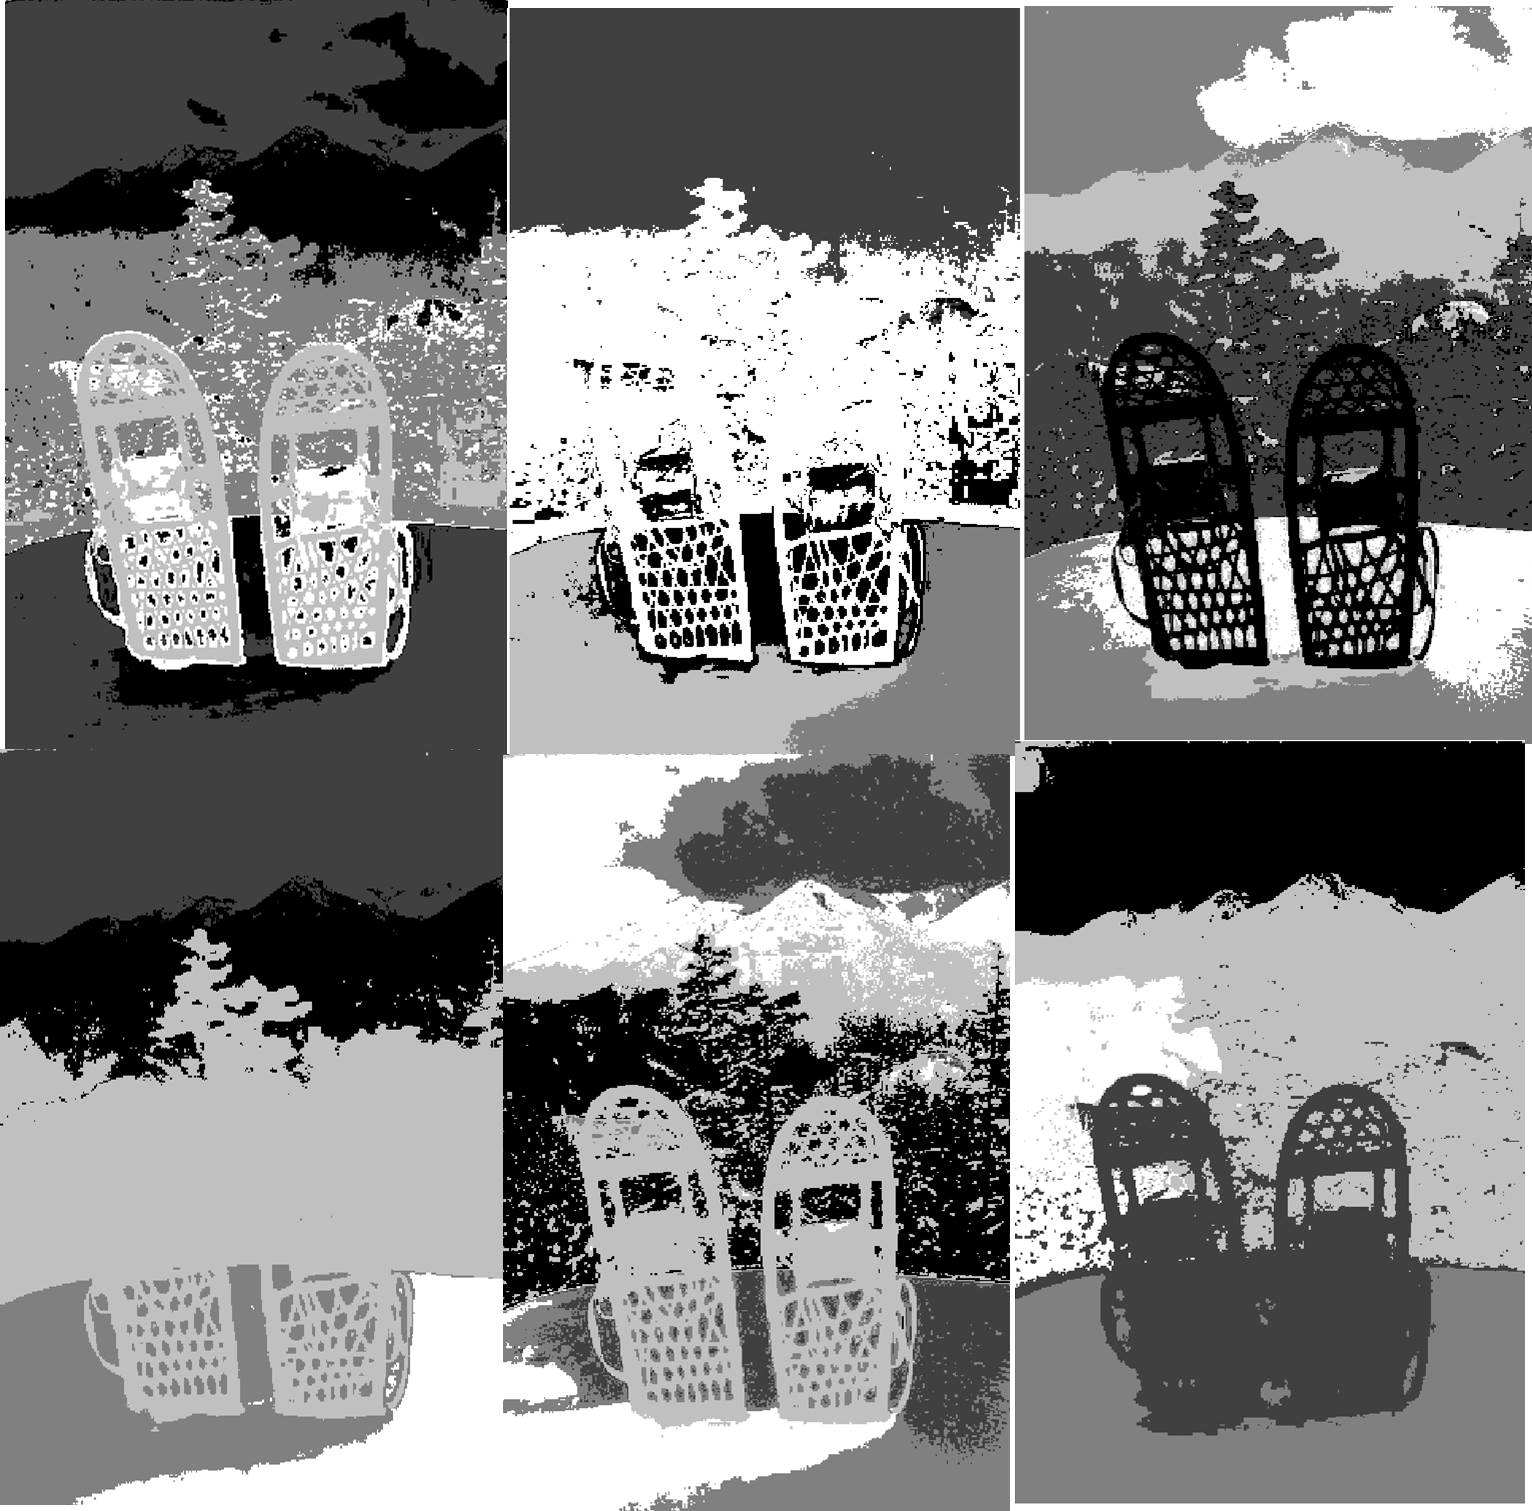
\includegraphics[width=0.4\textwidth]{Gmm.jpg}
    \caption{Segmentaciones por medio de GMM para diferentes representaciones con 5 clusters: De izquierda a derecha de arriba a abajo: HSV, HSV+XY, LAB, LAB+XY, RGB, RGB+XY.}
    \label{fig:gmm}
\end{figure}

\begin{figure}[h]
    \centering
    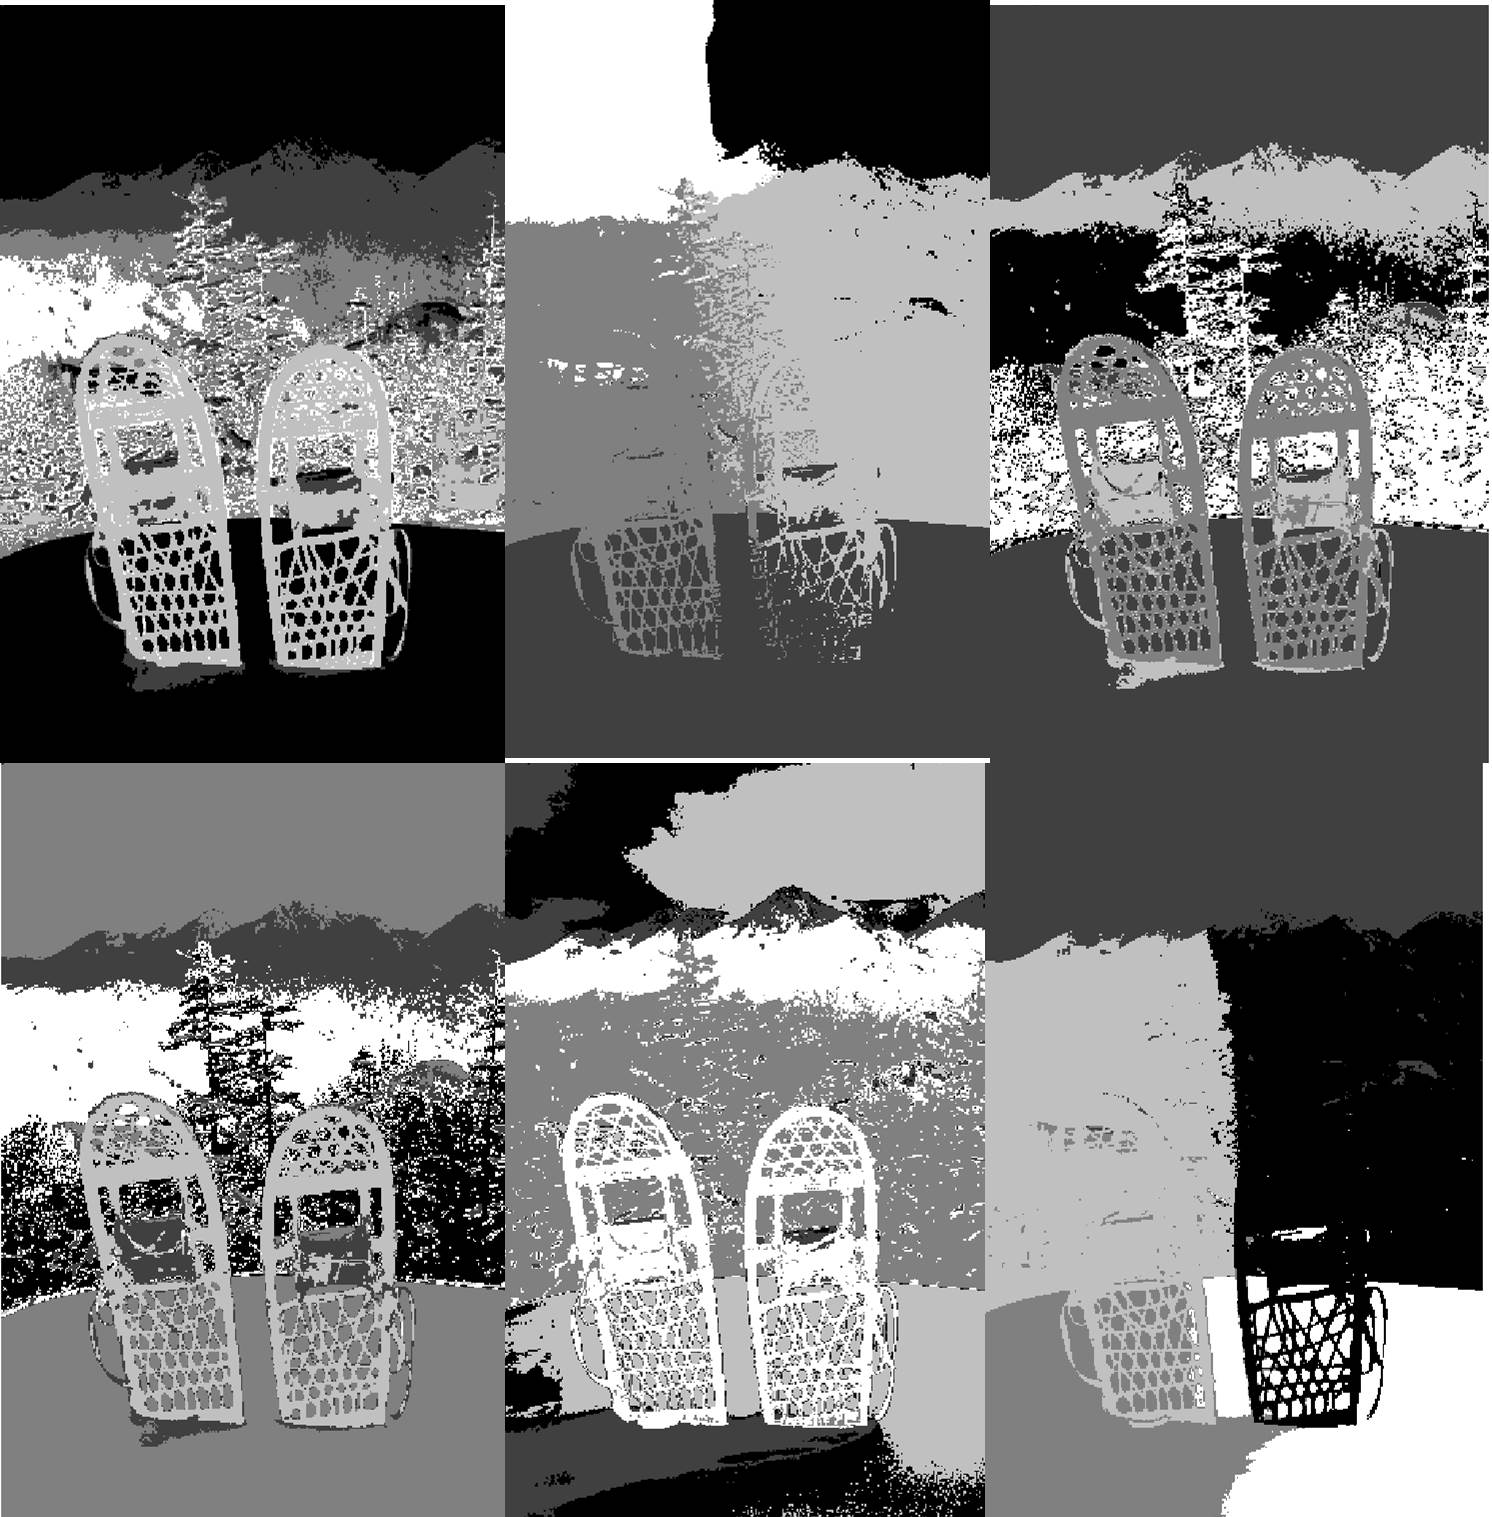
\includegraphics[width=0.4\textwidth]{Kmeans.jpg}
    \caption{Segmentaciones por medio de Kmeans para diferentes representaciones con 5 clusters: De izquierda a derecha de arriba a abajo: HSV, HSV+XY, LAB, LAB+XY, RGB, RGB+XY.}
    \label{fig:kmeans}
\end{figure}

\begin{figure}[h]
    \centering
    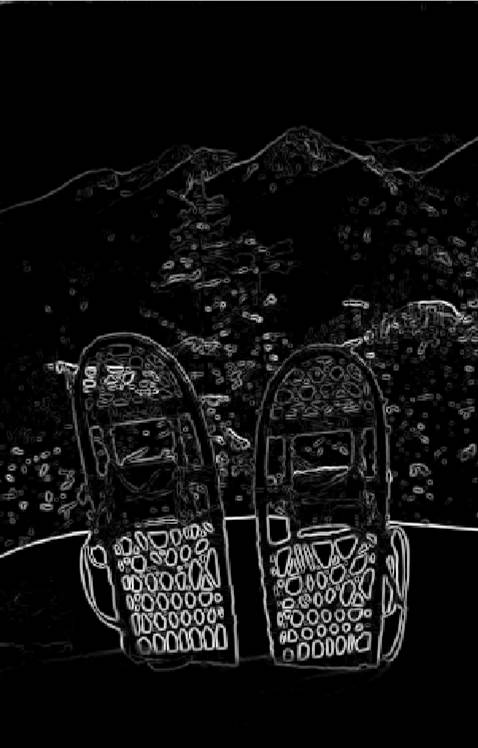
\includegraphics[width=0.2\textwidth]{Watersheds.jpg}
    \caption{Segmentación por medio de watersheds con mínimos regionales extendidos a nivel 50}
    \label{fig:watersheds}
\end{figure}

\subsection{Metodología de prueba}
La metodología de prueba se basó en camparar las segmentaciones construidas con las segmentaciones reales hechas por humanos de cada imágen. La función \textit{boundaryBench()} en matlab, propuesta por el grupo de Berkeley, realizó esta operación. Al comparar los bordes de las regiones anotadas por humanos con los bordes de las regiones obtenidas por las segmentaciones automáticas, se pueden calcular dos números que cuantifican lo buena o mala de la segmentación obtenida automáticamente:

\begin{equation} 
 Precisión=\frac{TP}{TP+FP}
\end{equation}
\begin{equation} 
 Cobertura=\frac{TP}{TP+FN}
\end{equation}

Donde FP=Falso positivo, TP=Verdadero positivo y FN=Falso negativo.

Cada segmentación se comparó con la segmentación real realizada por humanos obteniendo su precisión y cobertura. Al hacer esto con las \(200 \times 7 = 1400\) segmentaciones de cada combinación, se obtuvieron, por cada combinación, 7 puntos diferentes en la gráfica de precisión-cobertura (correspondientes a las precisiones y coberturas de las 200 imágenes sobre cada uno de los 7 niveles de segmentación) que se unieron en forma de curva sobre la gráfica. Al hacer esto con las tres combinaciones método/espacio de color, se obtuvieron tres curvas distintas que representan el desepeño de los métodos propuestos sobre la base de datos BSDS500. Se obtuvo también la curva para el método UCM a modo de comparación de los métodos básicos utilizados con un método mucho más avanzado en el área. Finalmente, a cada curva se le halló el \textit{F-measure}, que cuantifica cada método de manera más exacta.

\begin{equation}
 F=\frac{2(Precisión)(Cobertura)}{Precisión+Cobertura}
\end{equation}

Este valor corresponde a la comparación final entre los métodos estudiados y UCM.

%-------------------------------------------------------------------------
\section{Resultados}
Luego de hacer las segmentaciones con las tres combinaciones método/espacio de color (KMeans+RGB, KMeans+L*a*b* y Jerárquica+L*a*b*), se evaluaron las imágenes resultado según la metodología de evaluación explicada en la sección anterior. El resultado final de estos experimentos se muestra en la figura ~\ref{fig:resultados}

\begin{figure}[h]
    \centering
    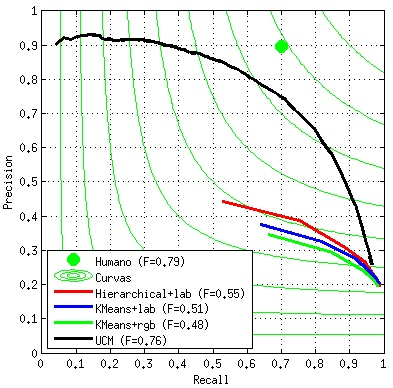
\includegraphics[width=0.5\textwidth]{PrecisionRecallComparativo.jpg}
    \caption{Resultado: gráfica precisión-cobertura para los diferentes métodos de segmentación}
    \label{fig:resultados}
\end{figure}

Se observan cuatro curvas distintas correspondientes a los cuatro métodos comparados. Aparte de esto se encuentra un punto verde con precisión de 0.9 y cobertura de 0.7, que corresponde a la evaluación sobre segmentaciones humanas. Las curvas verdes más delgadas son una especie de curvas de nivel, donde todo punto que se encuentre sobre una de esas curvas tiene el mismo \textit{F-measure}.

Es importante tener en cuenta que lo ideal en una gráfica de estas es llegar al punto (1,1), donde la precisión y la cobertura son máximas. En este caso, que se tiene comparación con la segmentación humana, se busca llegar a él con un método de segmentación automática.



%-------------------------------------------------------------------------
\section{Discusión}
Antes de desarrollar este experimento se tenían dos hipótesis principales: (1) los métodos de clustering básicos utilizados, como kmeans y jerárquico, deberían dar peores resultados en segmentación que un método más avanzado y desarrollado, como UCM y (2) en un problema de segmentación de imágenes por colores, como fue el caso de esta base de datos en este experimento, el espacio L*a*b* debería ser más adecuado que el espacio RGB para efectuar las segmentaciones. Los resultados de los experimentos comprueban dichas dos hipótesis sobre la base de datos BSDS500.

Estas dos conclusiones se obervan con las curvas en la figura ~\ref{fig:resultados}, viendo que hay un órden en las curvas. Si una curva es mayor a otra, quiere decir que el primer método es mejor que el segundo. Es claro que el punto verde es el ideal sobre la segmentación, ya que una segmentación automática que logre llegar a ese punto estaría igualando el nivel de la segmentación humana. Como el objetivo de la visión artificial es lograr algoritmos y mecanismos que permitan a computadores "ver como los humanos", este punto verde es, entonces, la misión en un problema de segmentación de imágenes. El \textit{F-measure} de la segmentación humana es 0.79 aproximadamente, mientras que el método UCM, propuesto por los investigadores de Berkeley alcanza un \textit{F-measure} de 0.76, lo cual demuestra que es un algoritmo muy bueno, alcanzando casi el desempeño humano. 

Los métodos intentados, como kmeans y segmentación jerárquica son métodos mucho más antiguos y básicos, por lo que se esperaba un menor desempeño a comparación con UCM. Esto fue observado. Bajo el espacio L*a*b*, la segmentación jerárquica obtuvo un \textit{F-measure} de 0.55 y la segmentación por kmeans de 0.51. Con esto también se pueden comparar los dos métodos evaluados, encontrando que la segmentación jerárquica es más eficiente para segmentación sobre esta base de datos. Esto se explica por varias razones: (1) la segmentación por kmeans suele crear clusters del mismo tamaño, mientras que la jerárquica no. En una imagen real los clusters no serán necesariamente del mismo tamaño; (2) la segmentación por kmeans suele crear clusters esféricos, a diferencia de la segmentación jerárquica que no busca una forma en específico; (3) la segmentación jerárquica crea una jerarquía de segmentaciones, por lo cual los grupos más grandes serán una combinación de los más pequeños, haciendo que los diferentes niveles de segmentación se encuentren anidados y sean más robustos, a diferencia de kmeans, donde cada nivel de segmentación es independiente; y (4) la segmentación por kmeans es altamente dependiente de la inicialización aleatoria de los centroides, haciendo que sea un método poco robusto, mientras que la jerárquica permite recrear mejor diferentes segmentaciones por la manera como se construye.

Aparte de esto fue posible comparar también el efecto del espacio de color empleado. Utilizando kmeans se comparó el resultado bajo codificación RGB y L*a*b*. Como fue mencionado anteriormente, se esperaba un mejor desempeño con L*a*b*, lo cual se evidenció. El \textit{F-measure} para RGB fue de 0.48, menor al 0.51 obtenido con L*a*b*. Este comportamiento se esperaba, porque el espacio L*a*b* es más acorde con la visión humana, ya que esta codificación es perceptualmente uniforme, lo cual significa que las distancias entre colores en la percepción humana se evidencian mejor en esa codificación que en RGB. Como la segmentación se hizo a partir del color de los píxeles, el espacio L*a*b* era más comprometedor.

Otra situación que se puede observar en la gráfica es que las curvas obtenidas por las tres combinaciones evaluadas son más cortass que las de UCM. La explicación de este fenómeno es que la curva de UCM se construyó con un número mucho mayor de niveles de segmentaciones. Por cuestiones de tiempo y memoria computacional se segmentó con las tres combinaciones con siete números distintos de clusters, haciendo que en evaluación estos métodos tengan menos niveles de segmentación que lo que se hizo con UCM, lo cual se traduce en gráficas más cortas. Aún así se evidencia la tendencia de las tres curvas a explicar que Jerárquico+L*a*b* es mejor que kmeans+L*a*b* y este a su vez es mejor que kmeans+RGB, siendo estos tres menos eficientes que UCM sobre la base de datos BSDS500. 

Un punto interesante en esta gráfica es que, mirándola desde la derecha, los tres métodos implementados empiezan casi sobre el mismo punto (precisión=0.2 y cobertura casi 1), lo cual significa que, bajo ese nivel de segmentación, hay una gran cantidad de detecciones (casi todas las anotaciones se detectan) pero con muy baja precisión (hay un número grande de falsos positivos, es decir, detecciones que no hacen parte de las anotaciones). El método UCM empieza cercano de ese punto pero con mejor precisión (un 0.05 mejor), mostrando que para ese nivel, la cantidad de falsos positivos es menor en ese método. UCM aumenta muy rápidamente a partir de ese punto, disminuyendo drásticamente los falsos positivos a medida que el nivel de segmentación disminuye, mientras que en las segmentaciones por kmeans y jerárquica, el crecimiento es más lento, observando una menor disminución en los falsos positivos. Para llegar a precisiones más altas se requiere que la gran mayoría de detecciones sean anotaciones de la verdad terreno, cosa que parece ser difícil con kmeans y segmentación jerárquica. Para problemas de segmentación, estos dos métodos no son los más recomendados.



%-------------------------------------------------------------------------
\section{Conclusiones y mejoras potenciales}

Tres métodos de segmentación fueron comparados en términos de desempeño según la gráfica de precisión-cobertura para la base de datos BSDS500. Los dos primeros métodos (kmeans y segmentación jerárquica) mostraron desempeños inferiores al método UCM (\textit{F-measure}=0.76), que es más avanzado. Entre los dos primeros métodos se encontró que el primero fue mejor, al obtener un \textit{F-measure} de 0.55 sobre  un \textit{F-measure} de 0.51 del segundo método. Todo esto sobre el espacio de color L*a*b*. 

Se comparó además el desempeño de la segmentación sobre esa base de datos de acuerdo al espacio de color utilizado, concluyendo que el espacio L*a*b* (\textit{F-measure}=0.51) es mejor para segmentación en color que el espacio RGB (\textit{F-measure}=0.48), ya que el primero es perceptualmente uniforme, lo cual lo hace más acorde con las anotaciones humanas.

El método UCM está muy cerca del \textit{F-measure} de las segmentaciones huamanas (\textit{F-measure}=0.79), por lo que se considera un método altamente eficiente para la segmentación de imágenes. La segmentación jerárquica y kmeans, como fueron presentados en este documento, no son muy recomendables para la segmentación de imáganes debido a la gran cantidad de falsos positivos presentes. La cantidad de falsos negativos es baja en todos los casos.

Teniendo en cuenta que hay métodos de segmentación de imágenes muy eficientes hoy en día, como UCM, es más recomendable utilizar esos algoritmos para ese tipo de problemas y no recurrir a kmeans o a segmentación jerárquica. Sin embargo, sería interesante realizar este mismo experimento con un mayor número de clusters para evaluar de manera más precisa los desempeños. Para esto se requeriría un computador con mayor velocidad y memoria. Si se quiere segmentar con kmeans o jerárquico, debido a su facilidad y simplicidad, es posible hacer algunas mejoras a estos métodos, como por ejemplo utilizar una codificación de píxeles que no sólo tenga en cuenta el color de ellos sino también la textura y hasta sus coordenadas; también se podrían combinar los resultados de estos dos algoritmos (kmeans y jerárquico) para lograr un método más robusto y que tome lo mejor de los dos. Esto se podría lograr pesando la segmentación de cada método por un valor o comparando las dos imágenes  segmentadas para ver cuáles regiones se mantienen en las dos segmentaciones, haciendo que dichas regiones sean más probablemente las reales según las etiquetas. 

%-------------------------------------------------------------------------


{\small
\bibliographystyle{plain}
\bibliography{mybib}{}
}

\end{document}
